% Copyright 2004 by Till Tantau <tantau@users.sourceforge.net>.
%
% In principle, this file can be redistributed and/or modified under
% the terms of the GNU Public License, version 2.
%
% However, this file is supposed to be a template to be modified
% for your own needs. For this reason, if you use this file as a
% template and not specifically distribute it as part of a another
% package/program, I grant the extra permission to freely copy and
% modify this file as you see fit and even to delete this copyright
% notice. 

\documentclass{beamer}
\usepackage{amsmath,amsfonts,amssymb,amsthm}
\usepackage{eqparbox}
\usepackage{textcomp}
\usepackage{blindtext}
\usepackage{textgreek}
\usepackage{gensymb}
\usepackage{xcolor}
\usepackage{color}
\usepackage{soul}
\usepackage{placeins}
\usepackage{graphics}
\usepackage{graphicx}
\usepackage{textpos}
\usepackage{caption}
\usepackage{color}
\usepackage{bm}
\usepackage{tikz}
\usepackage{pgf}
\captionsetup[figure]{labelformat=empty}
\graphicspath{{Figures/}}
\usepackage[natbib=true, style=numeric, sorting=none, backend=bibtex]{biblatex}
\addbibresource{MastersResults.bib}

% There are many different themes available for Beamer. A comprehensive
% list with examples is given here:
% http://deic.uab.es/~iblanes/beamer_gallery/index_by_theme.html
% You can uncomment the themes below if you would like to use a different
% one:
%\usetheme{AnnArbor}
%\usetheme{Antibes}
%\usetheme{Bergen}
%\usetheme{Berkeley}
%\usetheme{Berlin}
%\usetheme{Boadilla}
%\usetheme{boxes}
%\usetheme{CambridgeUS}
\usetheme{Copenhagen}
%\usetheme{Darmstadt}
%\usetheme{default}
%\usetheme{Frankfurt}
%\usetheme{Goettingen}
%\usetheme{Hannover}
%\usetheme{Ilmenau}
%\usetheme{JuanLesPins}
%\usetheme{Luebeck}
%\usetheme{Madrid}
%\usetheme{Malmoe}
%\usetheme{Marburg}
%\usetheme{Montpellier}
%\usetheme{PaloAlto}
%\usetheme{Pittsburgh}
%\usetheme[height=10mm]{Rochester}
%\usetheme{Singapore}
%\usetheme{Szeged}
%\usetheme{Warsaw}

%\useoutertheme[footline=authortitle]{miniframes}
\usecolortheme{default}

\title{Measurements of the Hardness Factor for Proton Beams of Various Energies.}

% A subtitle is optional and this may be deleted
%\subtitle{Cameron Simpson-Allsop}

\author{C. Simpson-Allsop, L. Ram, K. Nikolopoulos, T. Price, I. Mateu \vspace{-1cm}}
% - Give the names in the same order as the appear in the paper.
% - Use the \inst{?} command only if the authors have different
%   affiliation.
\date{University of Birmingham, \\ \vspace{0.1cm} October 12 2018}
% - Either use conference name or its abbreviation.
% - Not really informative to the audience, more for people (including
%   yourself) who are reading the slides online

% If you have a file called "university-logo-filename.xxx", where xxx
% is a graphic format that can be processed by latex or pdflatex,
% resp., then you can add a logo as follows:

% \pgfdeclareimage[height = 1cm]{logo}{Figures/UoB_logo.png}
% \logo{\pgfuseimage{logo}}
 
\titlegraphic{
\includegraphics[width=1.5cm]{UoB_logo.png}\hspace*{4.75cm}~%
   
\includegraphics[width=1.5cm]{ATLAS_logo.png}
}

\addtobeamertemplate{navigation symbols}{}{%
    \usebeamerfont{footline}%
    \usebeamercolor[fg]{footline}%
    \hspace{1em}%
    \insertframenumber/\inserttotalframenumber
}

\begin{document}
    \begin{frame}
      \titlepage
    \end{frame}

    \begin{frame}{Outline}
    The hardness factor ($\kappa$) of three different proton beams has been measured:
      \begin{itemize}
          \item MC40 Cyclotron (25 MeV)
          \item IRRAD Cyclotron (24 GeV)
          \item KIT Cyclotron (24 MeV)
      \end{itemize}
    \end{frame}
    
    \begin{frame}{MC40 Cyclotron Results}
    For the MC40 cyclotron, all data taking and analysis was done in Birmingham. A universal maximum depletion voltage value of -91V was used.
    \begin{figure}
        \centering
        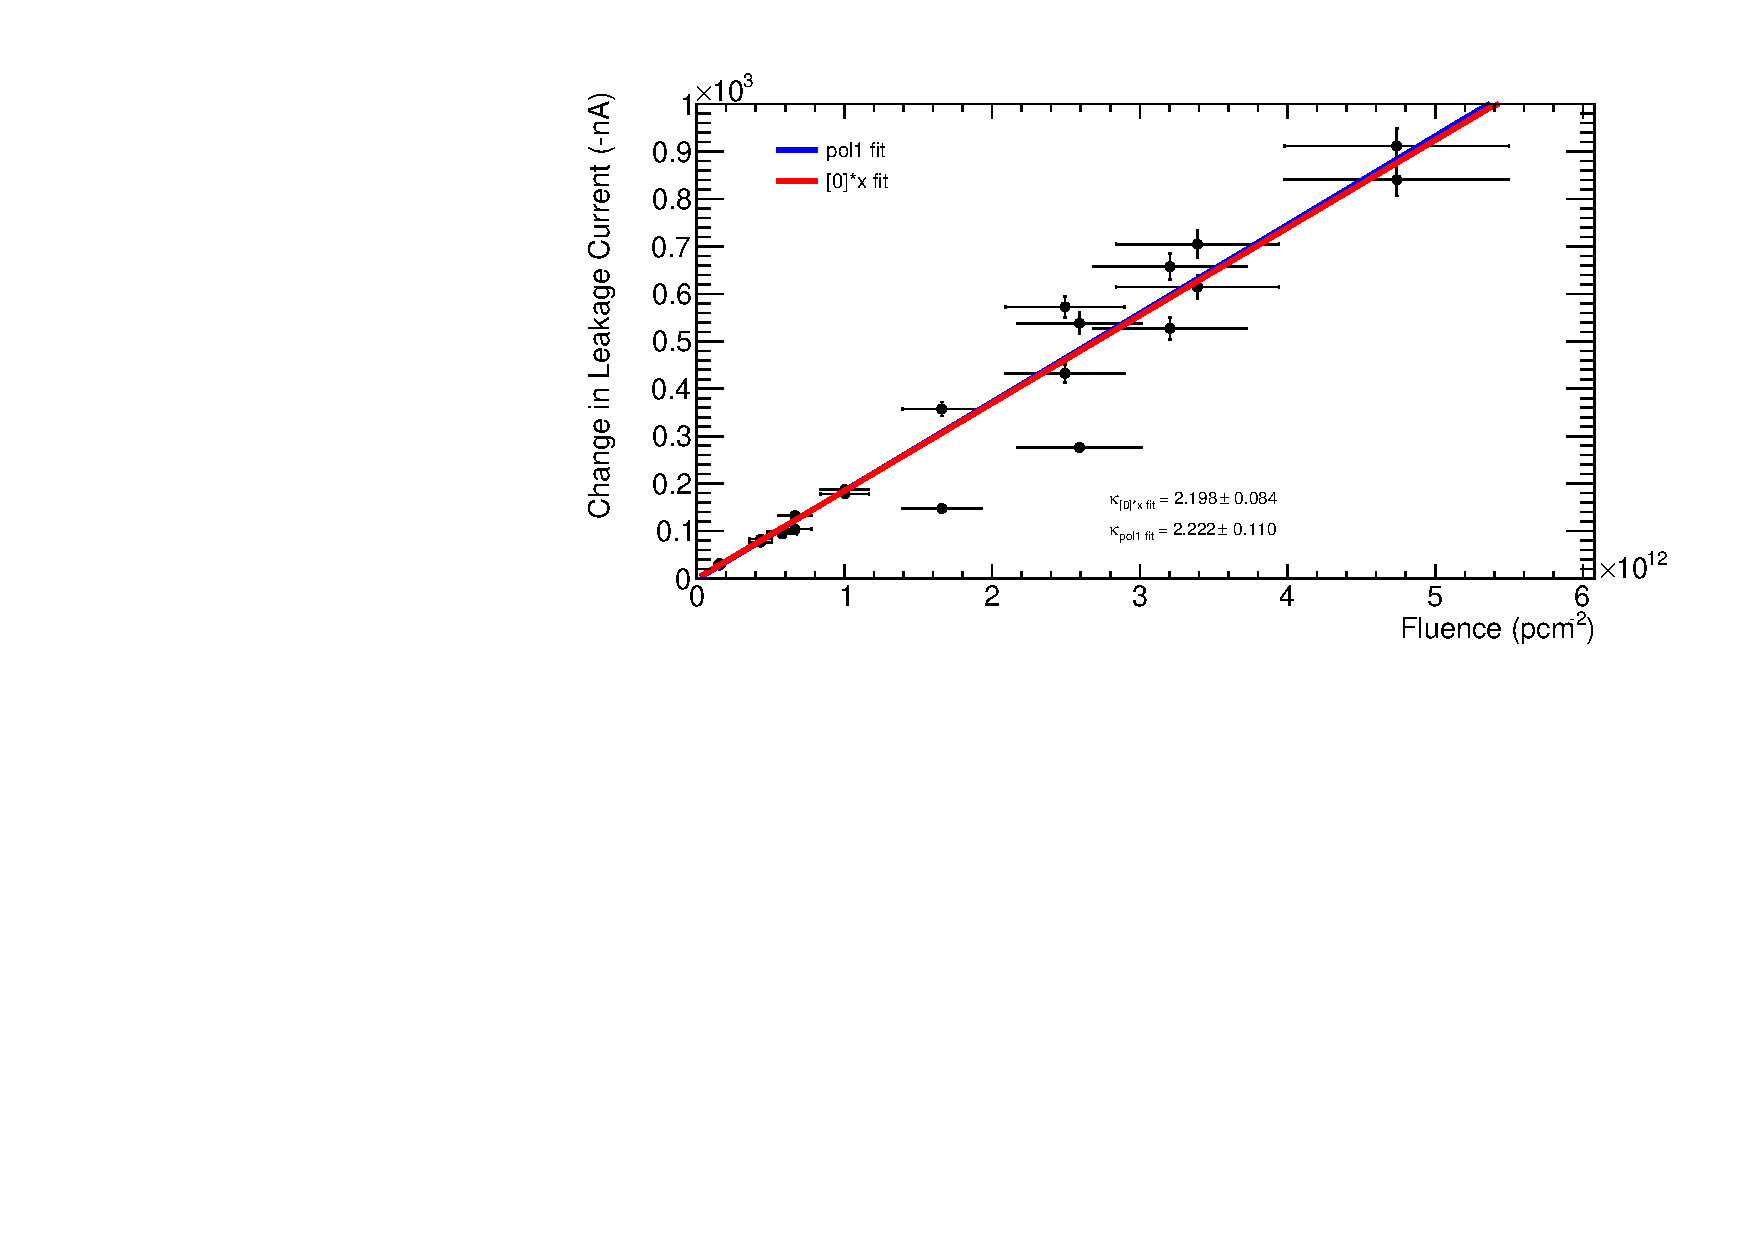
\includegraphics[width = 0.95\linewidth]{MC40.pdf}
    \end{figure}
    \end{frame}
    
    \begin{frame}{IRRAD Results}
    For IRRAD, all of the analysis was done in Birmingham, but the diodes were irradiated at IRRAD. As with the MC40 cyclotron, a universal maximum depletion voltage value of -91V was used.
        \begin{figure}
            \centering
            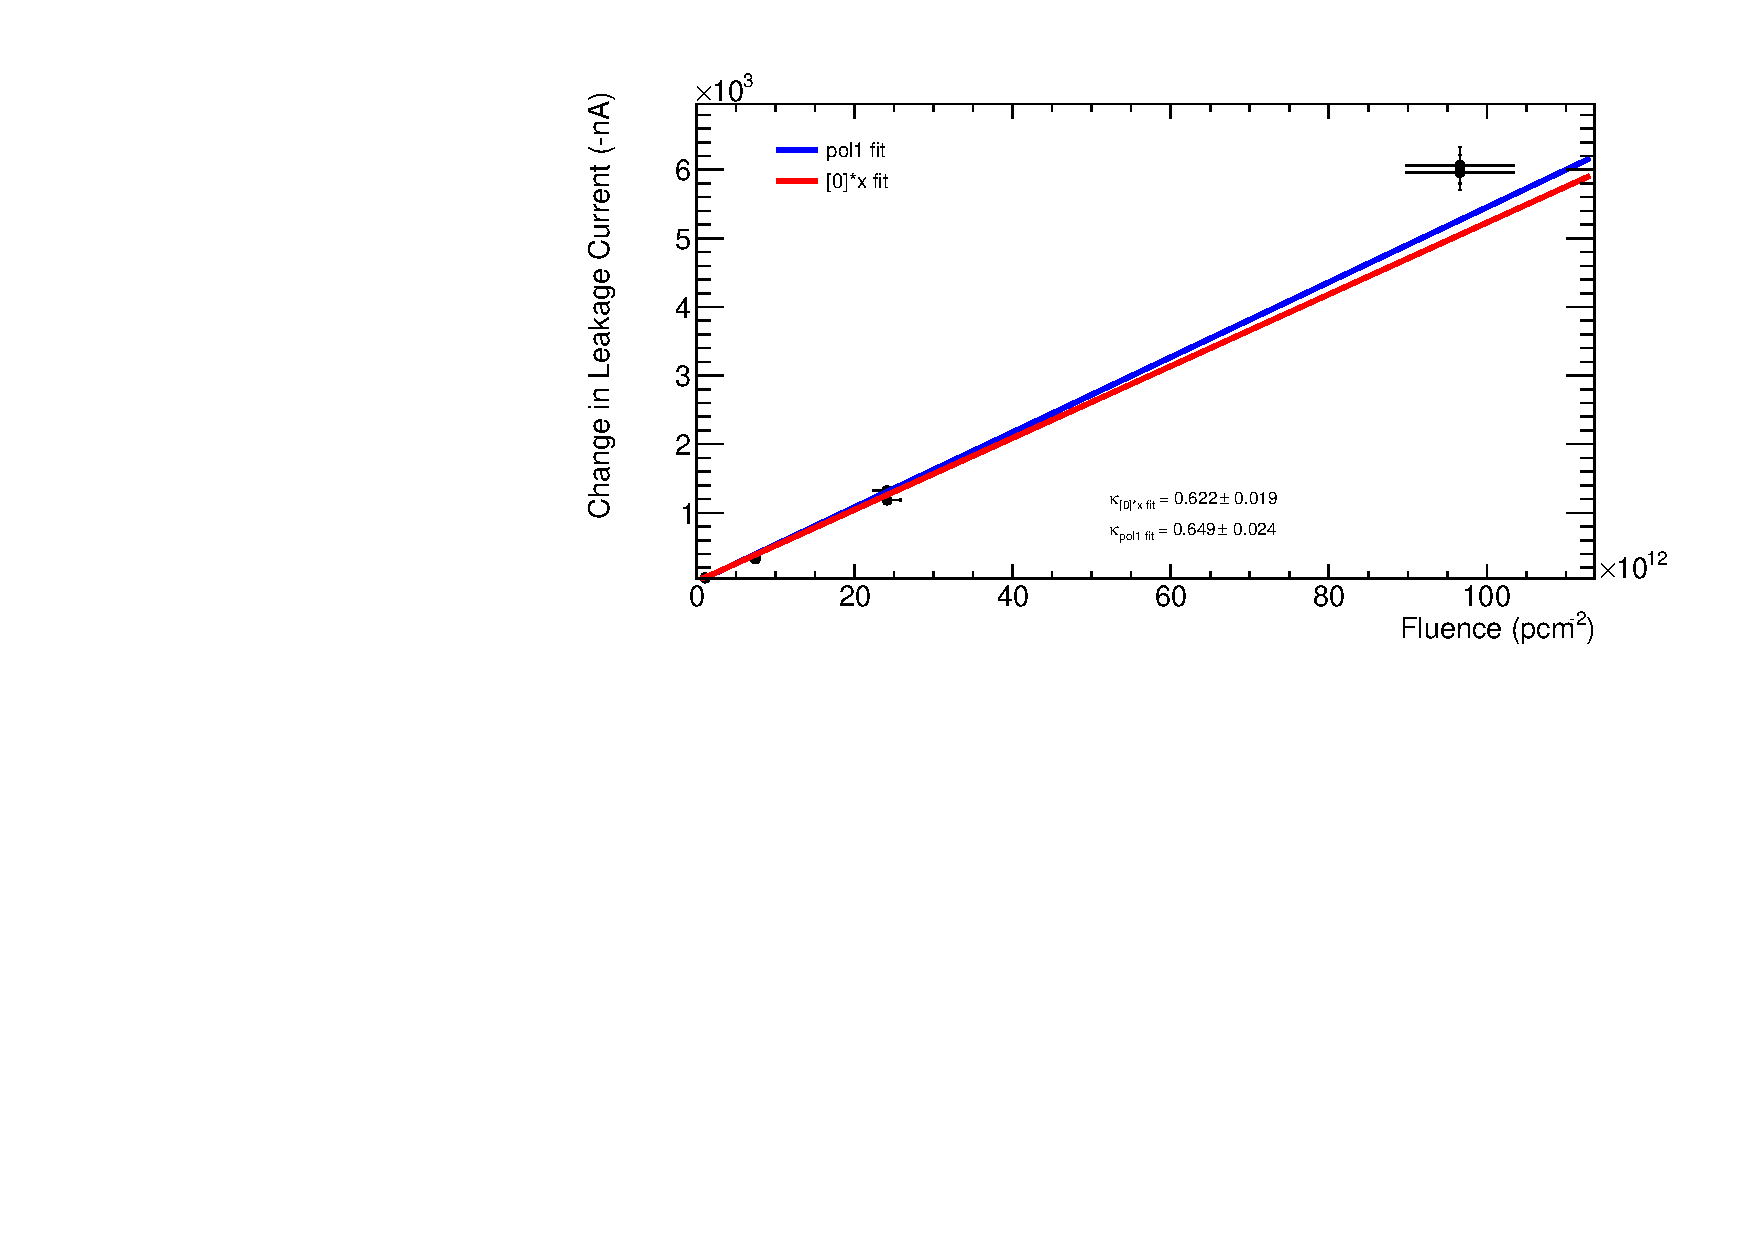
\includegraphics[width = 0.95\linewidth]{IRRAD.pdf}
        \end{figure}
    \end{frame}
    
    \begin{frame}{Isidre's Results}
    Isidre's data were taken completely independently for the IRRAD cyclotron, producing a value of $\kappa = 0.631 $. The data were then re-analysed in Birmingham as a cross check. The maximum depletion voltage in this case was individual for each data point.
        \begin{figure}
            \centering
            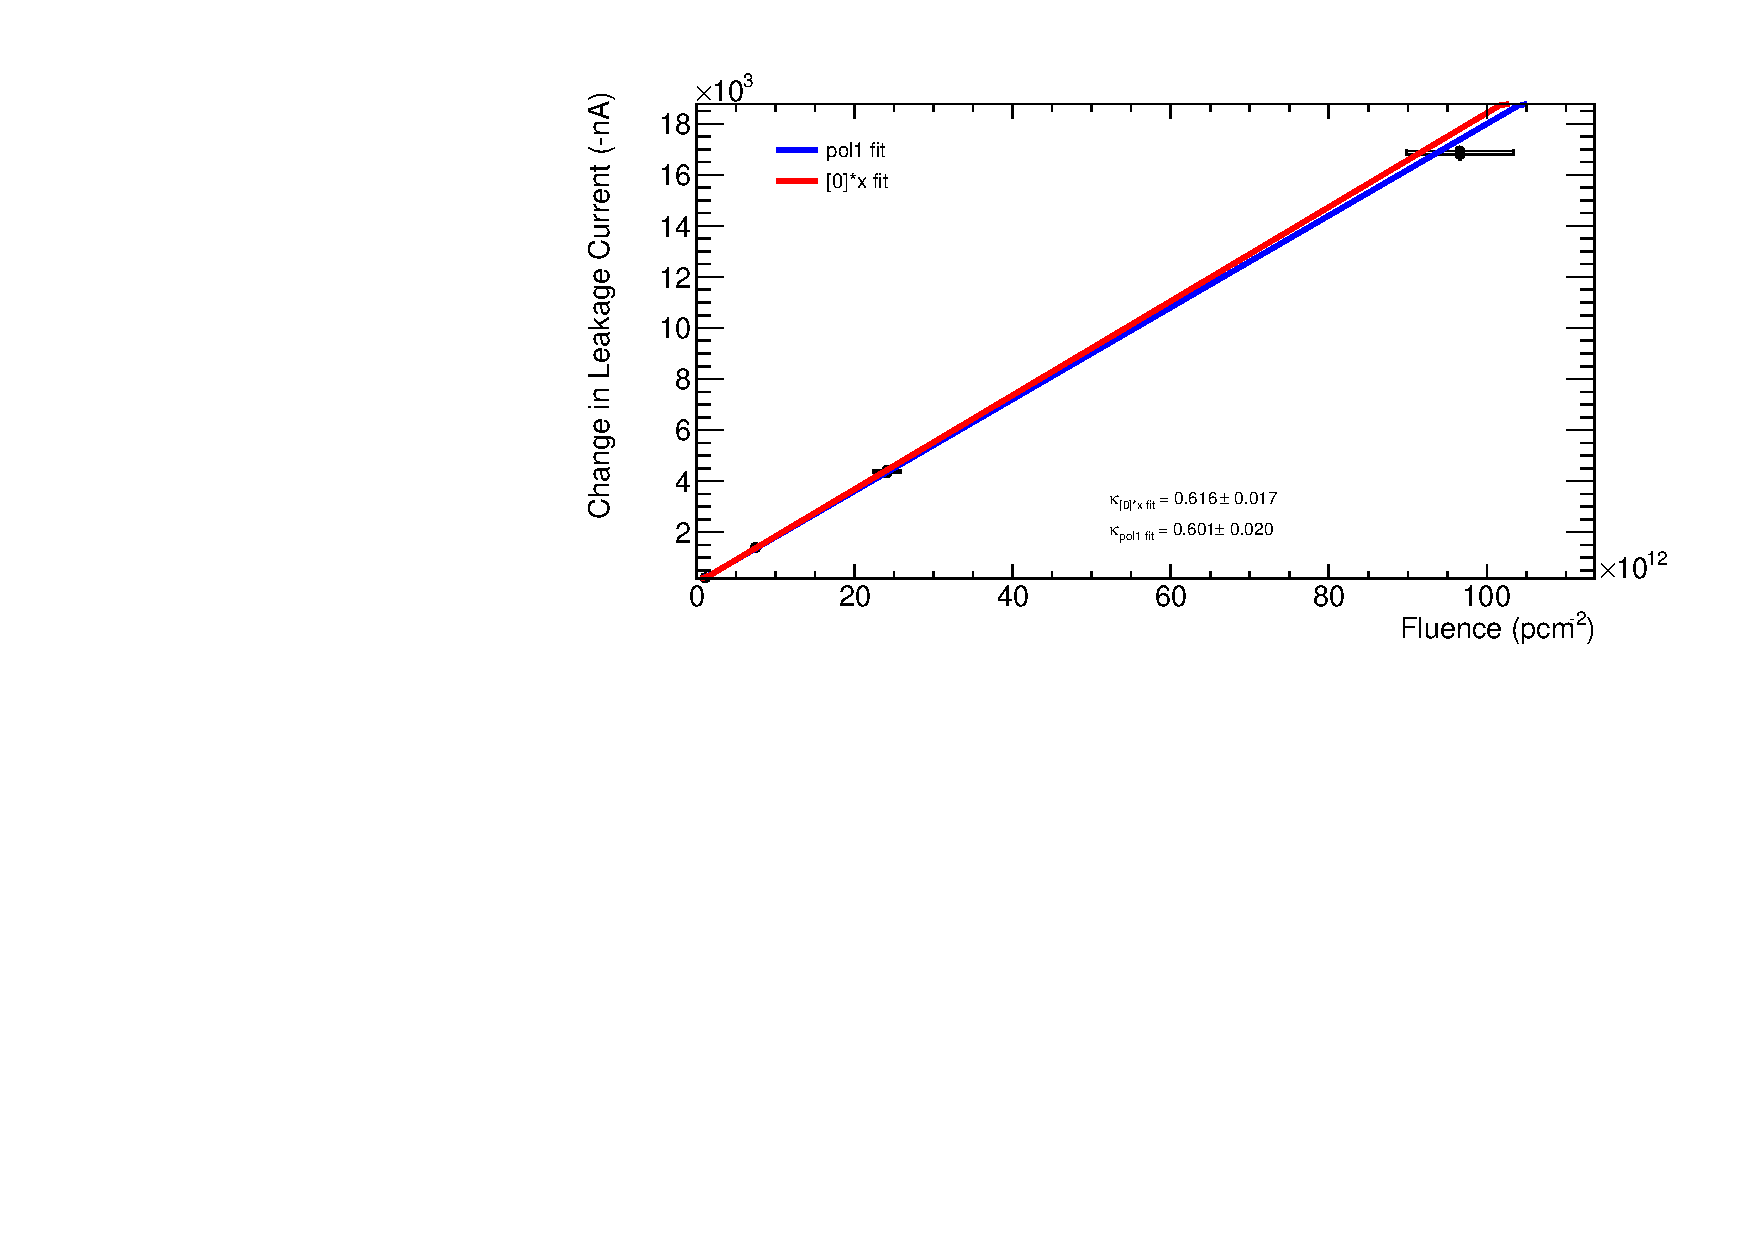
\includegraphics[width = 0.95\linewidth]{Isidre.pdf}
        \end{figure}
    \end{frame}
    
    \begin{frame}{Isidre's Results - CV example}
    Due to difficulty with fitting, instead of plotting logs, $1/C^2$ was plot against $V$, and the maximum depletion voltage for each sensor was determined by finding the intersect of the two fits.
        \begin{figure}
            \centering
            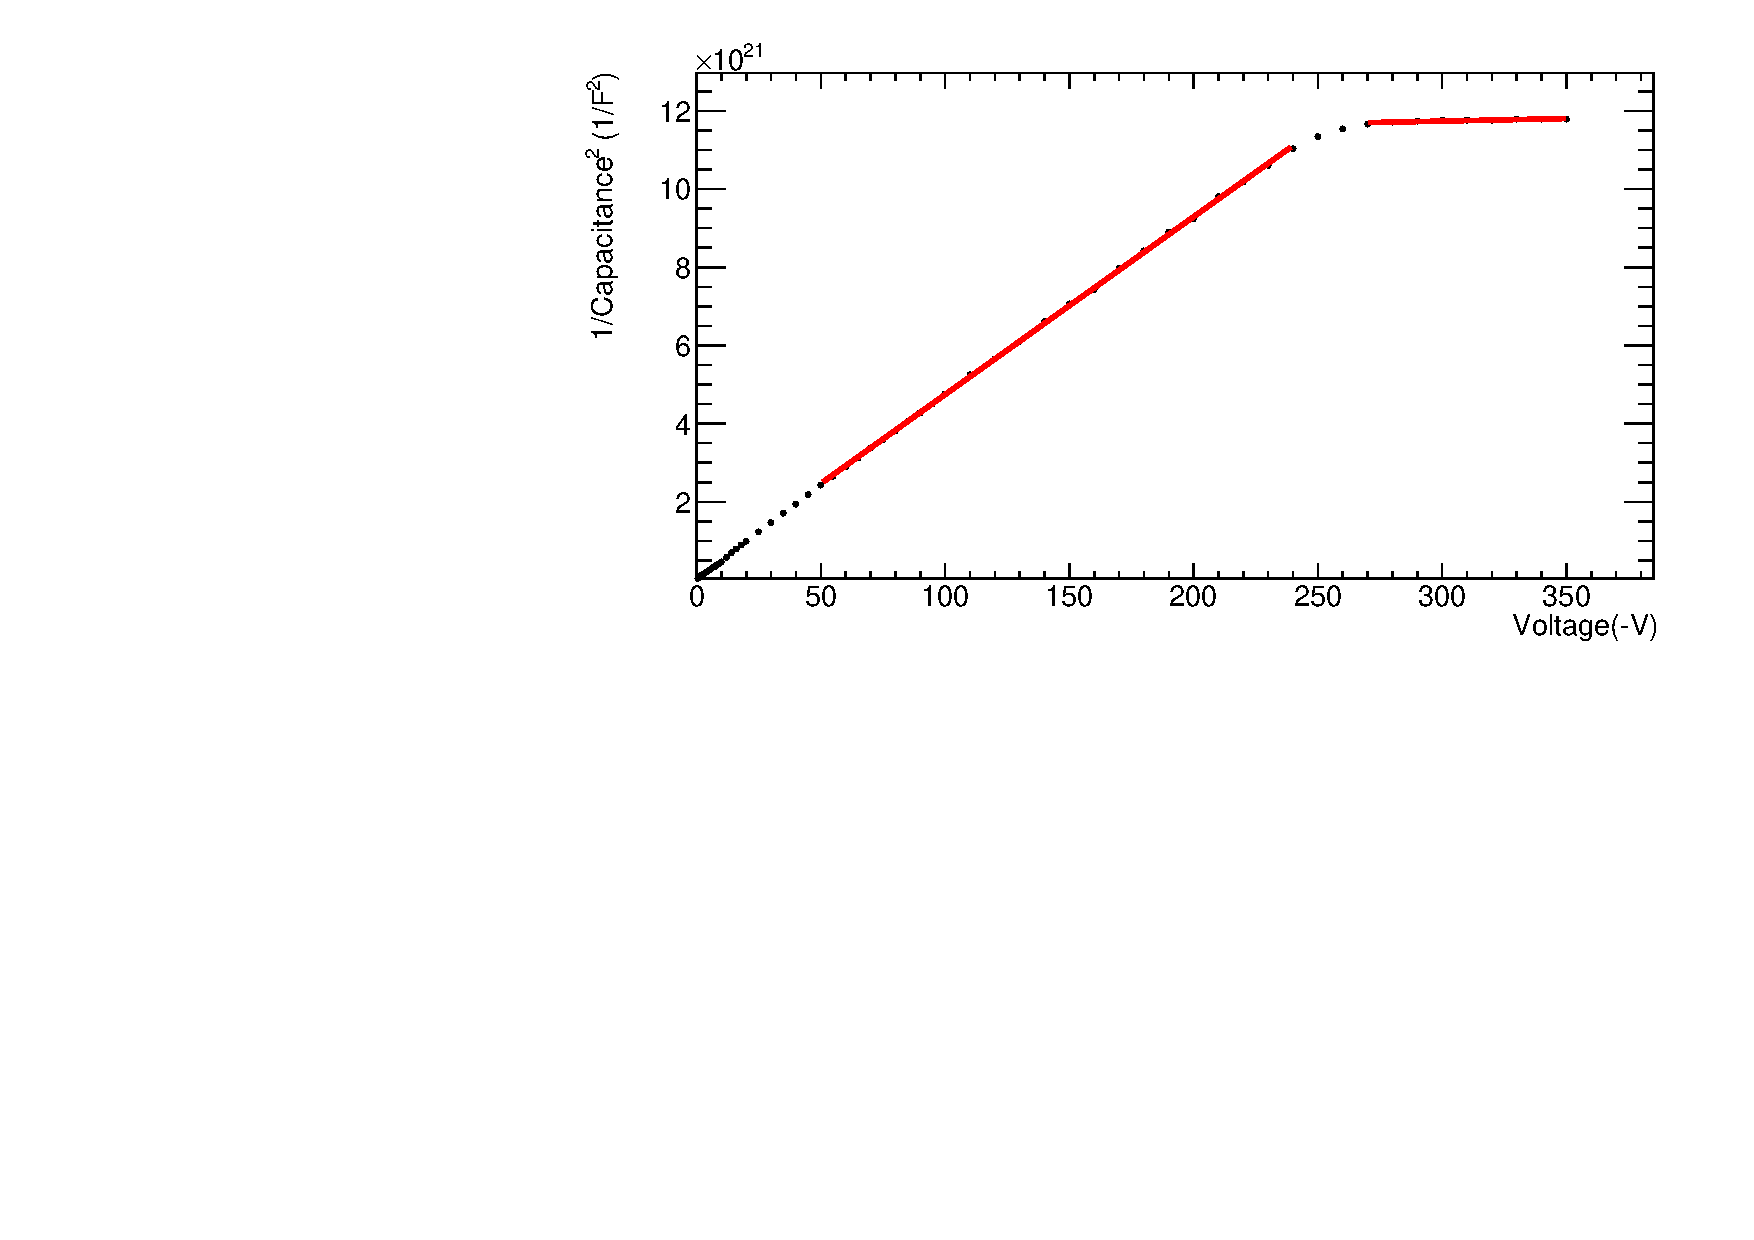
\includegraphics[width = 0.95\linewidth]{IsidreCVexample.pdf}
        \end{figure}
        
    \end{frame}
    
    \begin{frame}{KIT Results}
    For KIT, the diodes were irradiated in Karlsruhe, and then sent here for analysis. The only fit on this plot is a pol1 fit. The non-irradiated case was unknown, and so it was unjustified to force the fit through zero.
        \begin{figure}
            \centering
            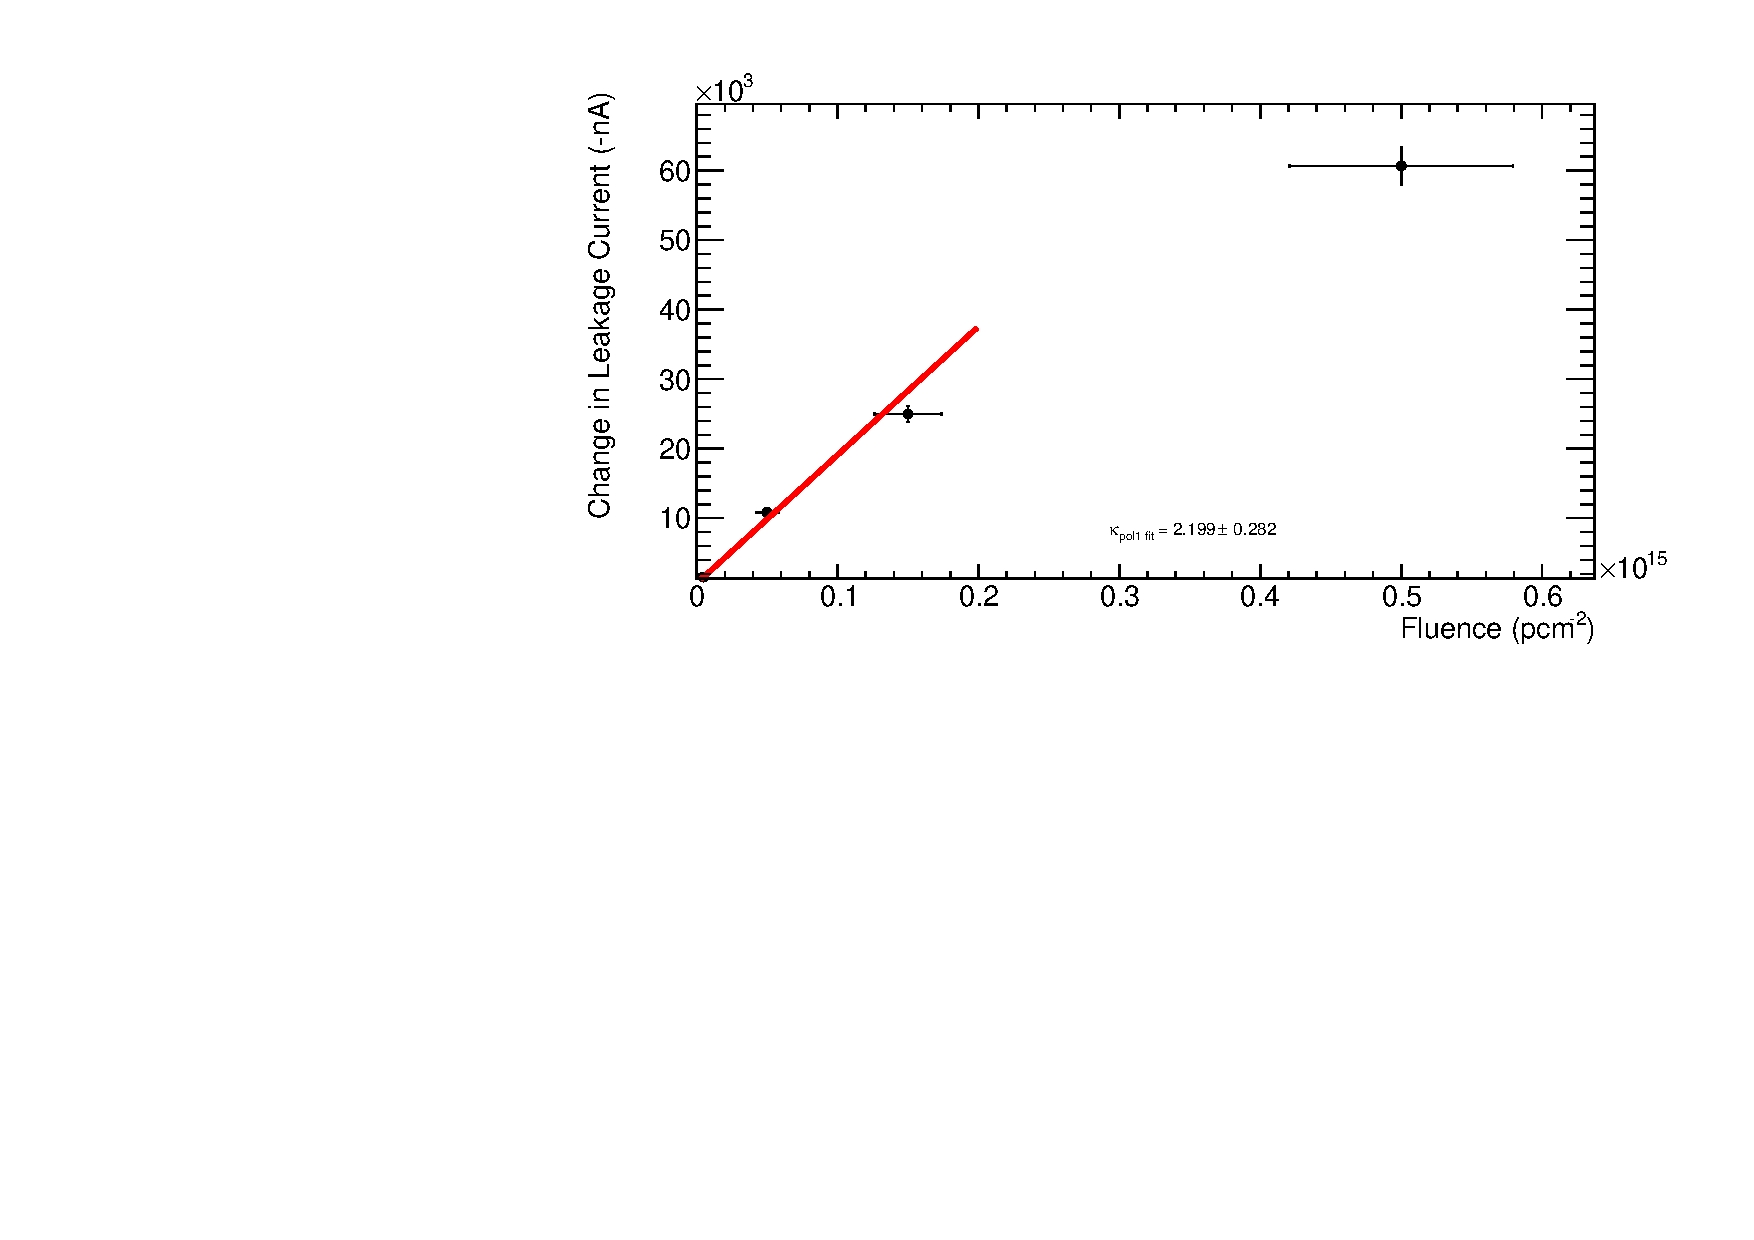
\includegraphics[width = 0.95\linewidth]{KIT.pdf}
        \end{figure}
    \end{frame}
    
    \begin{frame}{Conclusion}
    All values of $\kappa$ seem reasonable, and Isidre's results also seem to be in good alignment with ours.
        \begin{itemize}
            \item $\kappa _{MC40} = 2.20 \pm 0.08$
            \item $\kappa _{IRRAD} = 0.62 \pm 0.02$
            \item $\kappa _{Isidre} = 0.62 \pm 0.02$ (My analysis)
            \item $\kappa _{Isidre} = 0.63$ (Isidre's Analysis)
            \item $\kappa _{KIT} = 2.20 \pm 0.28$
        \end{itemize}
    Note: The values taken are from fits forced through zero (excluding the KIT result).
    \end{frame}

\end{document}


